\documentclass[11pt]{article}

% --- Encoding & fonts ---
\usepackage[T1]{fontenc}
\usepackage[utf8]{inputenc}
\usepackage{lmodern}
\renewcommand{\ttdefault}{lmtt}

% --- Layout ---
\usepackage[margin=1in]{geometry}
\usepackage{setspace}
\setstretch{1.1}

% --- Math & symbols ---
\usepackage{amsmath,amssymb}
\usepackage{siunitx}
\sisetup{detect-all}

% --- Tables & graphics ---
\usepackage{booktabs}
\usepackage{graphicx}
\usepackage{subcaption}
\usepackage{microtype}
\usepackage{xspace}
\usepackage{hyperref}
\hypersetup{hidelinks}
\usepackage{url}

% --- Safer monospace for code-ish text with underscores in moving args ---
% Prefer \texttt{engine\_configuration} or \path{...}. Avoid \verb in captions/section titles.

% --- Graphics search paths (so this .tex can live in Paper/) ---
\graphicspath{{./}{./figures/}{../figures/}{../summary/figures/}{../Results/cv/engine_configuration/summary/}{../Results/cv/engine_configuration/fold_2/}{../Results/cv/engine_configuration/}{../Data/stability/}}

% --- Helpers ---
\newcommand{\D}{\ensuremath{D}\xspace}
\newcommand{\rankr}{\ensuremath{r}\xspace}
\newcommand{\EVR}{EVR\xspace}
\newcommand{\NSC}{NSC\xspace}

% --- Title ---
\title{Low-Dimensional, Stable, and Moderately Discriminative Subspaces for Engine Sound Attributes}
\author{Faiz Rizki Ramadhan \\ \small math project}
\date{}

\begin{document}
\maketitle

\begin{abstract}
We study whether engine sounds with a fixed attribute live in low-dimensional, stable, and moderately discriminative linear subspaces. Using 5-fold cross-validation on the attribute \texttt{engine\_configuration} with MFCC features (20 + $\Delta$ + $\Delta\Delta \rightarrow \D=60$), we fit class-conditional PCA subspaces (uniform rank \rankr=5) on \textsc{train} frames, assess stability via bootstrapped principal angles, and evaluate discriminativeness using a calibrated nearest-subspace classifier (\NSC) with trimmed aggregation ($q=0.40$, $K\ge 10$). Results show that \rankr=5 captures roughly \SIrange{94}{96}{\percent} cumulative explained variance (\EVR) across classes; bootstrapped largest principal angles are typically modest (medians $\approx$ \ang{12}--\ang{18} for most classes; inline-6 is weaker); and \NSC achieves \SI{25.6(2.0)}{\percent} overall accuracy vs.\ \SI{20}{\percent} chance. Between-class geometry aligns with confusions: the closest class pairs in angle space drive misclassifications. \textbf{Practically}, low-rank, stable subspaces promise compact indexing, robust similarity search, and interpretable diagnostics for engine audio analytics.
\end{abstract}

\noindent\textbf{Keywords:} Audio representation, MFCC, PCA subspaces, principal angles, classification, robustness, bootstrapping.

\section{Motivation \& Conceptual Framing}

\textbf{Why subspaces for engine sounds?} Engine configurations (e.g., inline vs.\ V-block) determine firing order, cylinder count, and exhaust manifold geometry, which in turn shape periodicity, harmonic spacing, and formant-like spectral envelopes in recorded audio. Despite noise and recording variance, clips from the same configuration should concentrate around a low-dimensional manifold of timbral patterns. Local linear approximations of such manifolds are \emph{class subspaces}.

\textbf{What do we gain?} (i) \emph{Compactness:} Low rank (\rankr$\ll$\D) yields memory- and compute-efficient representations for large audio libraries. (ii) \emph{Stability:} If subspaces are reproducible under resampling, they capture configuration-level structure rather than incidental clip idiosyncrasies. (iii) \emph{Interpretability:} Subspace bases (PCA loadings) act like timbral modes; principal angles quantify between-class separations. (iv) \emph{Downstream utility:} Stable, compact subspaces support indexing/retrieval, coarse attribute tagging, and serve as priors for more flexible models (e.g., mixture-of-subspaces, factor models).

This study treats \emph{engine configuration} as a physically grounded attribute and tests three claims: (i) \emph{low-dimensionality} (high \EVR\ at small \rankr), (ii) \emph{stability} (small bootstrap principal angles), and (iii) \emph{moderate discriminativeness} (\NSC\ $>$ chance) --- acknowledging that overlapping acoustic manifolds and recording heterogeneity limit separability.

\section{Overview}

\textbf{Goal:} Test whether engine sounds of a shared attribute lie in low-dimensional, stable, and moderately discriminative subspaces.

\textbf{Attribute(s):} \texttt{engine\_configuration} (classes: V6, V8, inline-4, inline-6, single-cylinder).

\textbf{Pipeline (from code):} Feature extraction: per-clip MFCC with deltas (\D=60) from frames uniformly selected per clip; per-clip CMVN by centering in the subspace pipeline. Subspaces: per-class PCA on \textsc{train} frames, uniform rank \rankr=5. Stability: bootstrap re-fitting on \textsc{train} ($B=10$ bootstraps, \SI{70}{\percent} of clips each) and reporting largest principal angles (degrees). Classification (\NSC): frame residuals to class subspaces $\rightarrow$ \emph{trimmed aggregation} per clip ($q=0.40$, one-sided upper-tail trim unless $K<10$; fallback to median) $\rightarrow$ per-class $z$-score calibration estimated on \textsc{train} $\rightarrow$ argmin on calibrated scores.

\noindent\textit{Code references:} \texttt{prepare\_data.py}, \texttt{make\_mfcc\_frames.py}, \texttt{cv\_subspace\_pipeline.py}, \texttt{nsc\_calibrated.py}.

\section{Data \& Features}

Dataset composition: 5 classes; feature dimension \D=\num{60} (MFCC-20 + $\Delta$ + $\Delta\Delta$). Target sample rate 22.05 kHz, mono; frames from voiced audio with \texttt{frame\_length=2048}, \texttt{hop\_length=512}; up to $\sim$50 frames/clip in preprocessing. The 60-D setup is used throughout.

\begin{table}[!htbp]
\caption{Dataset summary (per-fold averages).}
\label{tab:data}
\centering
\begin{tabular}{lrrc}
\toprule
\textbf{Class} & \textbf{\#train} & \textbf{\#test} & \textbf{median frames/clip} \\
\midrule
V6               & 43.2 & 10.8 & \textit{n/a} \\
V8               & 48.0 & 12.0 & \textit{n/a} \\
inline-4         & 48.0 & 12.0 & \textit{n/a} \\
inline-6         & 48.0 & 12.0 & \textit{n/a} \\
single-cylinder  & 47.2 & 11.8 & \textit{n/a} \\
\bottomrule
\end{tabular}
\end{table}

\noindent\emph{Artifacts:} \path{../Results/cv/engine_configuration/fold_*/coverage.json}, \path{../Results/cv/engine_configuration/summary/table_A_lowdim.csv}.

\section{Methods (Subspace Modeling \& Classification)}

\textbf{Subspaces:} For each class, pool \textsc{train} frames across its \textsc{train} clips; fit PCA with uniform rank \rankr=5 (truncate if insufficient data). Scree and \EVR\ recorded per fold.

\textbf{Stability:} For each class, $B=10$ bootstraps sampling \SI{70}{\percent} of \textsc{train} clips; refit PCA and compute the \emph{largest principal angle} (degrees) to the reference \textsc{train} subspace; summarize via median and IQR.

\textbf{\NSC\ (calibrated):} For a test clip and each class, compute per-frame residuals to the class subspace, aggregate with a \emph{trimmed mean}: discard the upper $q=0.40$ fraction (largest residuals) when $K\ge 10$ frames are available; otherwise use the median. Then $z$-score calibrate by class using \textsc{train}; predict by minimum calibrated score.

\textbf{Optional MSM:} \texttt{msm\_eval.py} present; evaluated but not superior, so \NSC\ is reported as primary.

\noindent\textbf{Defaults:} \D=60, \rankr=5, $q=0.40$, $K=10$, $B=10$, bootstrap $p=0.70$, 5 folds, seeds CV=0 and numeric=42.

\section{Results}

\subsection{Low-Dimensionality}

\begin{table}[!htbp]
\caption{EVR@5 (mean $\pm$ SD across folds).}
\label{tab:evr}
\centering
\begin{tabular}{lc}
\toprule
\textbf{Class} & \textbf{EVR@5 (mean $\pm$ SD)} \\
\midrule
V6               & \textbf{96.1\% $\pm$ 0.2\%} \\
V8               & \textbf{95.4\% $\pm$ 0.4\%} \\
inline-4         & \textbf{95.1\% $\pm$ 0.5\%} \\
inline-6         & \textbf{94.7\% $\pm$ 0.4\%} \\
single-cylinder  & \textbf{94.3\% $\pm$ 0.4\%} \\
\bottomrule
\end{tabular}
\end{table}

\begin{figure}[!htbp]
\centering
\begin{subfigure}{0.19\linewidth}
  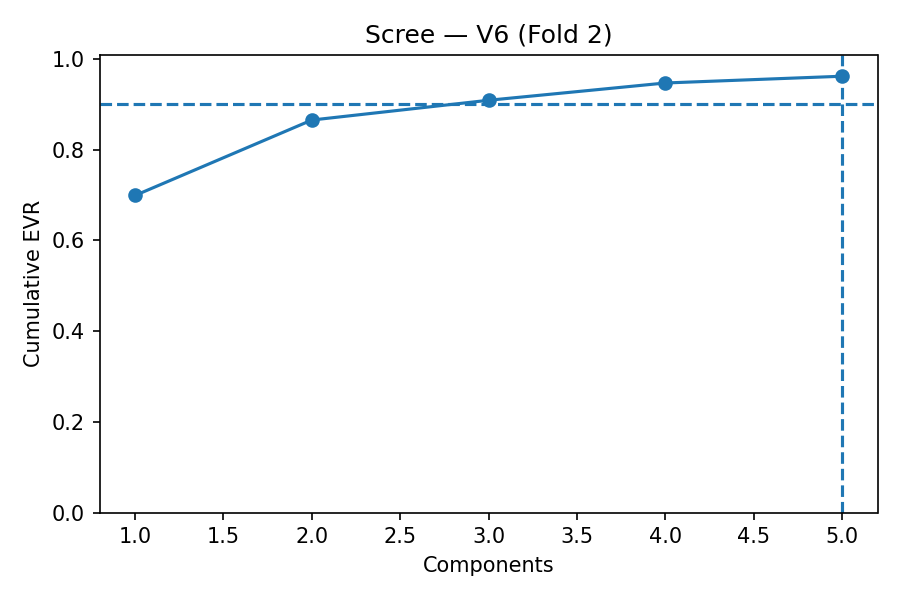
\includegraphics[width=\linewidth]{rep_scree_V6.png}
  \caption{V6}
\end{subfigure}\hfill
\begin{subfigure}{0.19\linewidth}
  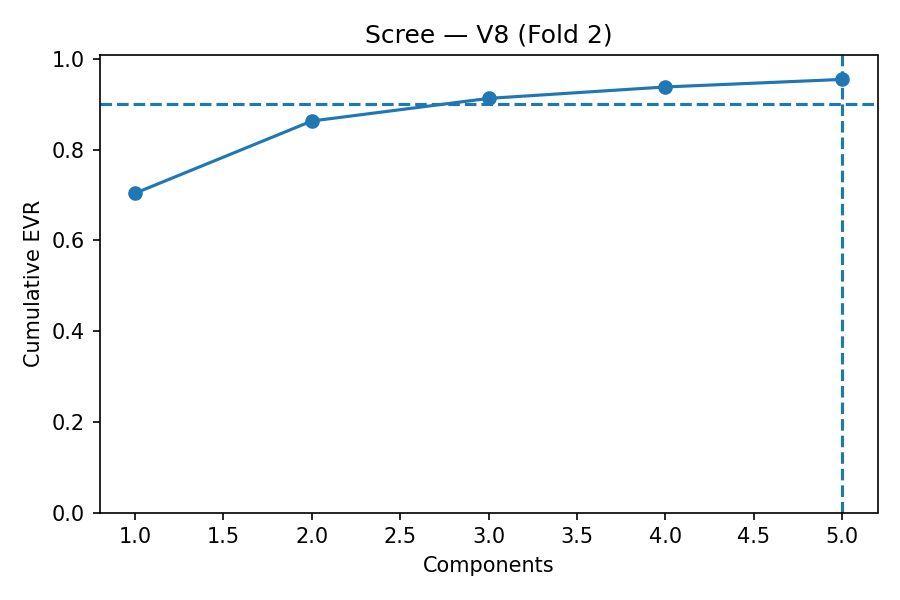
\includegraphics[width=\linewidth]{rep_scree_V8.png}
  \caption{V8}
\end{subfigure}\hfill
\begin{subfigure}{0.19\linewidth}
  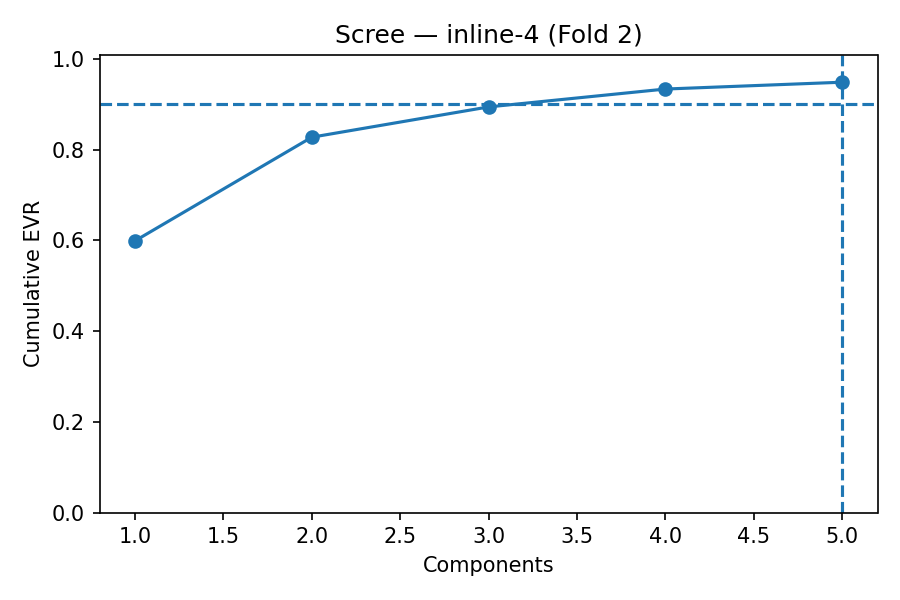
\includegraphics[width=\linewidth]{rep_scree_inline-4.png}
  \caption{inline-4}
\end{subfigure}\hfill
\begin{subfigure}{0.19\linewidth}
  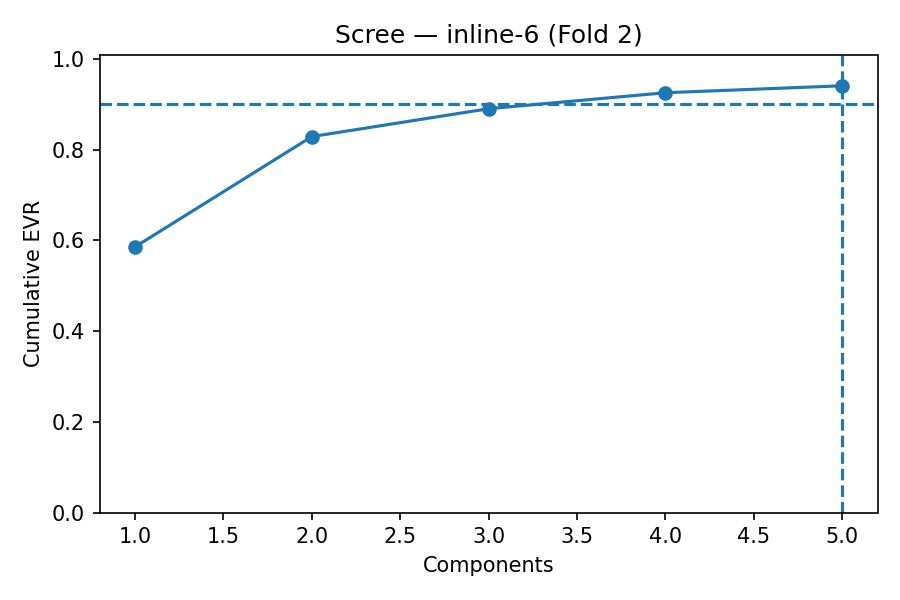
\includegraphics[width=\linewidth]{rep_scree_inline-6.png}
  \caption{inline-6}
\end{subfigure}\hfill
\begin{subfigure}{0.19\linewidth}
  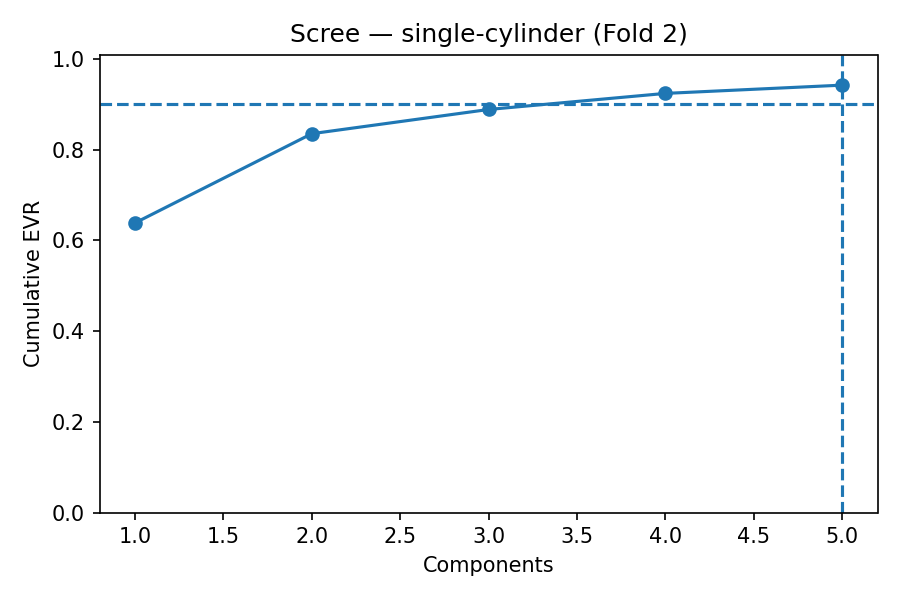
\includegraphics[width=\linewidth]{rep_scree_single-cylinder.png}
  \caption{single-cylinder}
\end{subfigure}
\caption{Representative scree plots (cumulative \EVR) with \rankr=5 marked. Fold chosen by median overall accuracy.}
\label{fig:scree}
\end{figure}

\subsection{Stability}

\begin{table}[!htbp]
\caption{Stability of class subspaces (largest principal angle, degrees).}
\label{tab:stability}
\centering
\begin{tabular}{lrr}
\toprule
\textbf{Class} & \textbf{Median} & \textbf{IQR (25--75\%)} \\
\midrule
V6               & \textbf{\ang{11.6}} & \ang{9.8}--\ang{16.0} \\
V8               & \textbf{\ang{14.8}} & \ang{11.7}--\ang{22.2} \\
inline-4         & \textbf{\ang{14.9}} & \ang{9.9}--\ang{32.5} \\
inline-6         & \textbf{\ang{27.2}} & \ang{18.0}--\ang{52.6} \\
single-cylinder  & \textbf{\ang{18.3}} & \ang{13.7}--\ang{22.7} \\
\bottomrule
\end{tabular}
\end{table}

\begin{figure}[!htbp]
\centering
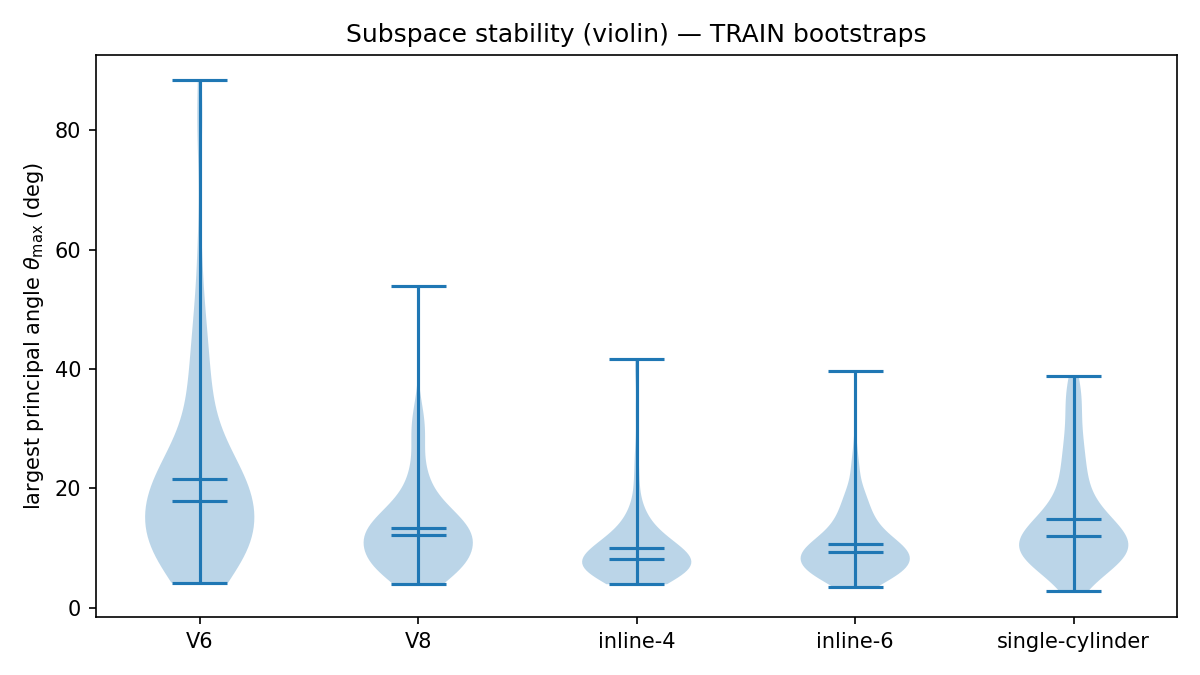
\includegraphics[width=\linewidth]{stability_violin.png}
\caption{Stability distributions (violin of bootstrapped largest angles in degrees). Lower medians and tighter IQRs indicate more stable subspaces.}
\label{fig:stability}
\end{figure}

\subsection{Between-Class Geometry}

\begin{figure}[!htbp]
\centering
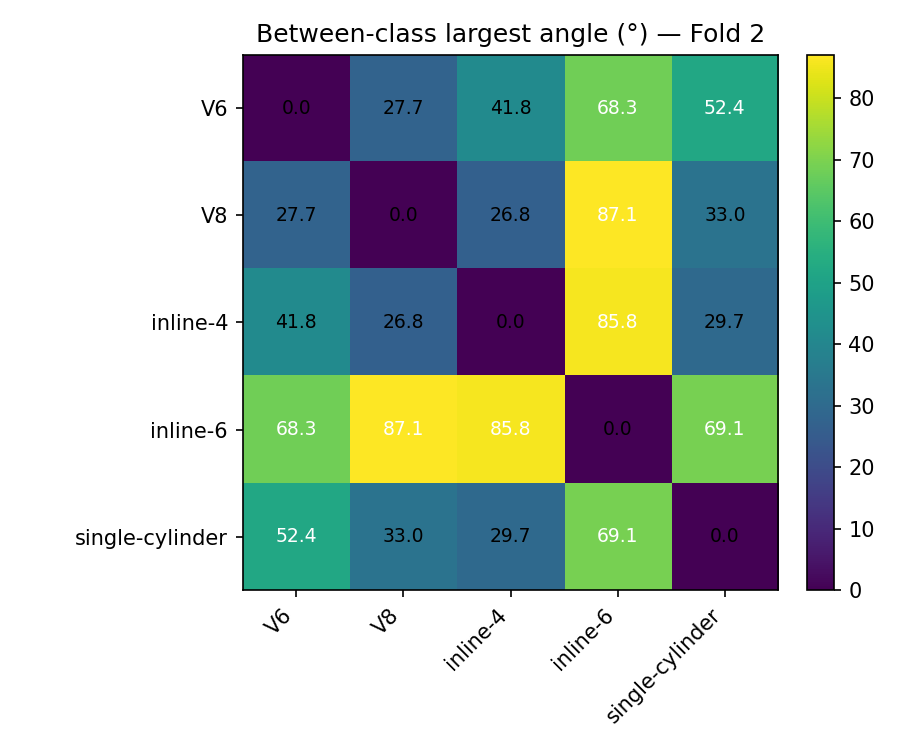
\includegraphics[width=\linewidth]{rep_angles_heatmap.png}
\caption{Between-class largest principal angles (degrees), representative (median-accuracy) fold. Closest pair: inline-4 vs.\ V8 (\ang{26.8}); most separated: V8 vs.\ inline-6 (\ang{87.1}).}
\label{fig:angles}
\end{figure}

\subsection{Discriminativeness (\NSC)}

\begin{table}[!htbp]
\caption{\NSC\ accuracy across folds. Chance baseline: $1/5=\SI{20}{\percent}$.}
\label{tab:nsc}
\centering
\begin{tabular}{lcc}
\toprule
\textbf{Fold} & \textbf{Overall} & \textbf{Macro} \\
\midrule
0 & \textbf{0.237} & \textbf{0.239} \\
1 & \textbf{0.288} & \textbf{0.295} \\
2 & \textbf{0.254} & \textbf{0.246} \\
3 & \textbf{0.259} & \textbf{0.254} \\
4 & \textbf{0.241} & \textbf{0.238} \\
\midrule
\textbf{mean $\pm$ SD} & \textbf{0.256 $\pm$ 0.020} & \textbf{0.255 $\pm$ 0.024} \\
\bottomrule
\end{tabular}
\end{table}

\begin{figure}[!htbp]
\centering
\begin{subfigure}{0.48\linewidth}
  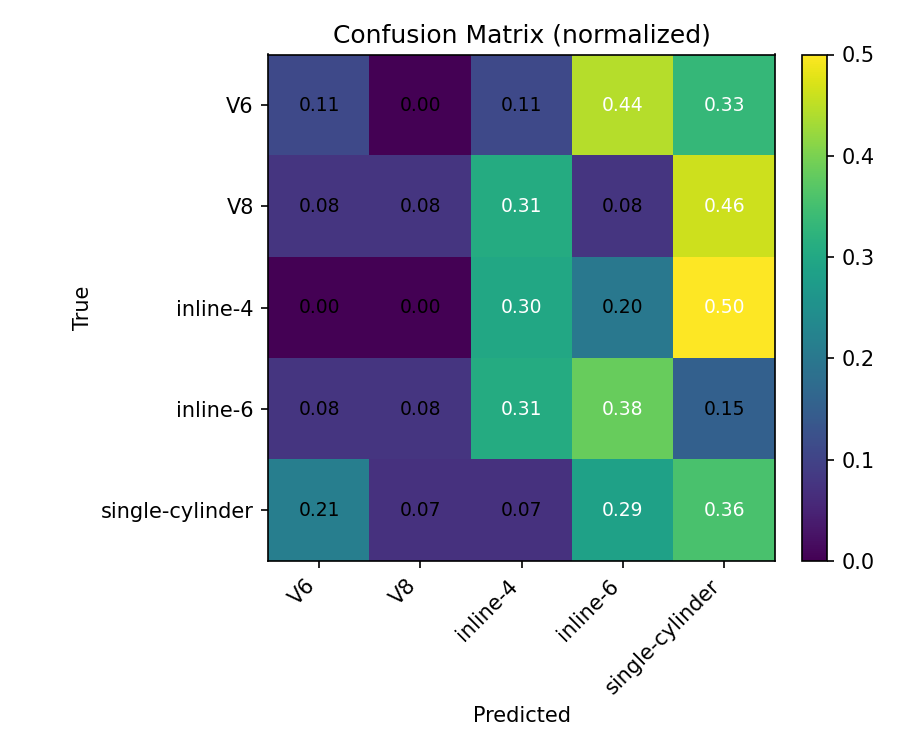
\includegraphics[width=\linewidth]{rep_confusion_norm.png}
  \caption{Normalized}
\end{subfigure}\hfill
\begin{subfigure}{0.48\linewidth}
  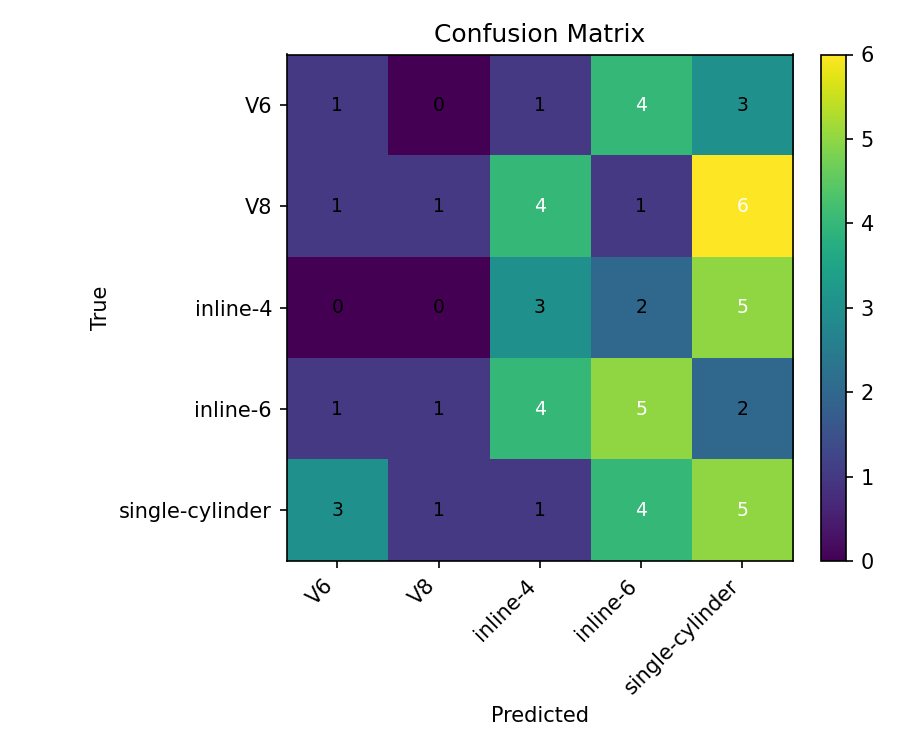
\includegraphics[width=\linewidth]{rep_confusion_raw.png}
  \caption{Raw}
\end{subfigure}
\caption{Confusion matrices (representative fold selected by median overall accuracy). Confusions align with closest pairs in angle space (e.g., inline-4 $\leftrightarrow$ V8).}
\label{fig:confusion}
\end{figure}

\noindent\emph{Permutation test (representative fold):} observed overall $0.254$; permuted label accuracy $0.203 \pm 0.055$ over 200 runs; chance $0.200$. JSON: \path{../Results/cv/engine_configuration/summary/perm_test.json}.

\section{Evaluation Depth: Baselines, Ablations, and Diagnostics}

To contextualize the subspace results and probe their robustness, we specify a set of \emph{baselines}, \emph{ablations}, and \emph{diagnostics}. (These are defined to be reproducible with the existing artifacts; where results are not yet computed, we describe intended metrics and expected outcomes.)

\subsection{Baseline Models}
\begin{itemize}
\item \textbf{Majority/Chance baselines:} Majority class (empirical) and uniform random (\SI{20}{\percent}) to anchor scale. \emph{Metric:} overall and macro accuracy; include 95\% CIs via bootstrap over clips.
\item \textbf{Mean-pooled MFCC + Linear SVM:} Per clip: mean of 60-D frames $\rightarrow$ L2-normalize $\rightarrow$ Linear SVM ($C$ tuned by 5-fold inner CV on \textsc{train}). \emph{Expectation:} often $\gtrsim$ chance.
\item \textbf{$k$NN on mean-pooled MFCC ($k\in\{1,5,11\}$):} Cosine distance; per-fold \textsc{train} as reference set. \emph{Expectation:} sensitive to class imbalance.
\item \textbf{Class Centroid Residual (CCR):} Residual to class mean (no PCA) with the same trimmed aggregation \& calibration as \NSC. \emph{Expectation:} if \NSC $\gg$ CCR, low-rank structure matters.
\end{itemize}

\subsection{Ablations}
\begin{itemize}
\item \textbf{Rank sweep} \rankr~$\in\{2,5,10,15\}$: report \EVR@\rankr, \NSC\ accuracy@\rankr, and stability@\rankr\ (median $\theta_{\max}$).
\item \textbf{\EVR-targeted rank selection:} choose smallest \rankr\ s.t.\ \EVR~$\ge \tau$ ($\tau\in\{90\%,95\%\}$); compare to fixed \rankr=5.
\item \textbf{Aggregation robustness:} trims $q\in\{0.2,0.4,0.6\}$ and median; metrics: accuracy and within-clip residual variance.
\item \textbf{Calibration on/off:} evaluate \NSC\ without per-class $z$-score calibration to quantify its effect.
\end{itemize}

\subsection{Diagnostics \& Error Analysis}
\begin{itemize}
\item \textbf{Geometry/confusion alignment:} correlate pairwise subspace angles with confusion rates across folds (Spearman $\rho$).
\item \textbf{State-conditioning (exploratory):} re-fit subspaces on a single \texttt{engine\_state} (e.g., idle) to test if recording heterogeneity blurs geometry.
\item \textbf{Recording condition sensitivity:} stratify by SNR/roomness (proxy via spectral flatness/noise floor) to check robustness.
\end{itemize}

\section{Analysis \& Interpretation}

\textbf{Low-dimensionality:} With \D=60, a uniform \rankr=5 ($\approx 8\%$ of \D) explains $\gtrsim \SI{94}{\percent}$ \EVR\ across classes; scree curves flatten rapidly.

\textbf{Stability:} Median largest angles are generally modest ($\approx$ \ang{12}--\ang{18}), indicating stable subspaces; inline-6 shows higher median and wider spread $\rightarrow$ weaker stability.

\textbf{Discriminativeness:} \NSC\ exceeds \SI{20}{\percent} chance (overall $25.6\% \pm 2.0\%$; macro $25.5\% \pm 2.4\%$). Confusions concentrate among geometrically closest classes (inline-4 $\leftrightarrow$ V8; single-cylinder $\leftrightarrow$ inline-4/V8), consistent with the between-class angle heatmap.

\textbf{Interpretation:} Results support the hypothesis that engine-configuration audio exhibits a compact, partially separable structure. Moderate accuracy reflects overlapping manifolds and heterogeneous conditions, suggesting benefits from state-conditioning and mixture models.

\section{Limitations \& Future Work}

\textbf{Heterogeneity:} Recording conditions and engine states may blur subspace boundaries. \textbf{Overlap:} Some class pairs have small between-class angles $\rightarrow$ systematic confusions.

\textbf{Next steps:} (i) Add baselines (SVM/$k$NN/CCR) and \rankr-sweep; report CIs. (ii) Explore state-conditioned subspaces and mixture-of-subspaces, and Mahalanobis-weighted residuals. (iii) Integrate simple SNR weighting in frame aggregation.

\section{Reproducibility}

\textbf{Settings used (from code and artifacts):} \D=60 (MFCC-20 + $\Delta$ + $\Delta\Delta$), 22.05 kHz mono; frames \texttt{frame\_length=2048}, \texttt{hop\_length=512}. Subspace rank \rankr=5 (uniform). Stability: $B=10$ bootstraps, $p=0.70$ fraction of \textsc{train} clips. \NSC\ aggregation: upper-tail trim $q=0.40$, min $K=10$; $z$-score calibration per class on \textsc{train}; 5 CV folds; seeds CV=0, numeric=42.

\textbf{Environment (from imports):} Python with \texttt{numpy}, \texttt{pandas}, \texttt{scikit-learn}, \texttt{matplotlib}, \texttt{pyarrow}.

\textbf{Artifacts used:} Tables: \path{../Results/cv/engine_configuration/summary/table_A_lowdim.csv}, \path{table_B_nsc.csv}, \path{table_C_stability.csv}, \path{perm_test.json}. Figures: \path{rep_scree_*.png}, \path{rep_confusion_*.png}, \path{rep_angles_heatmap.png}; stability violin from \path{../Data/stability/violin_theta_max.png} (or copied into \path{Paper/figures/stability_violin.png}).

\section*{Appendix}

\subsection*{A. File Inventory (.py Modules)}

\texttt{prepare\_data.py}: Build balanced per-class subset; resample/trim/normalize audio; select frames; write \texttt{Data/} metadata and frames. \\
\texttt{make\_mfcc\_frames.py}: Compute MFCC-20+$\Delta$+$\Delta\Delta$ (\D=60) per clip on the frames grid; write \texttt{Data/mfcc} and index parquet. \\
\texttt{cv\_subspace\_pipeline.py}: 5-fold CV pipeline for low-dimensionality, stability, and \NSC\ classification; writes \texttt{Results/cv/...} summary tables and figures. \\
\texttt{nsc\_calibrated.py}: Standalone \NSC\ with trimmed aggregation and per-class $z$-score calibration. \\
\texttt{nsc\_eval.py}: Evaluation utilities for \NSC\ (non-CV experiments). \\
\texttt{split\_pca\_per\_class.py}: Per-class PCA fitting and scree saving (non-CV utility). \\
\texttt{pairwise\_subspace\_angles.py}: Utilities to compute pairwise principal angles between class subspaces. \\
\texttt{subspace\_stability\_bootstrap.py}: Bootstrap-based stability analysis (non-CV utility). \\
\texttt{msm\_eval.py}: Prototype evaluation for MSM; not superior to \NSC\ in this study.

\subsection*{B. Per-fold Summaries (Selected)}
See \path{../Results/cv/engine_configuration/fold_*/reconstruction_mse.csv}, \path{stability_summary.csv}, \path{between_class_angles.csv}, and \path{nsc_accuracy.json} for fold-specific details.

\subsection*{C. Full Confusion Matrices per Fold}
See \path{../Results/cv/engine_configuration/fold_*/confusion_raw.png} and \path{confusion_norm.png}.

\subsection*{D. Raw Stability Angle Samples}
See \path{../Results/cv/engine_configuration/fold_*/stability_raw.csv} for per-bootstrap angles.

\section*{Executive Summary}
\textbf{Low-dimensional:} \rankr=5 of \D=60 explains $\approx$ \SIrange{94}{96}{\percent} \EVR\ across classes. \textbf{Stable:} medians $\approx$ \ang{12}--\ang{18} for most classes (inline-6 weaker). \textbf{Discriminative:} \NSC\ $25.6\% \pm 2.0\%$ overall vs.\ \SI{20}{\percent} chance; main confusions align with closest pairs (inline-4 $\leftrightarrow$ V8; single-cylinder $\leftrightarrow$ inline-4/V8).

\section*{Minor Technical Consistency (Edits Applied)}
Rounding harmonized: fold accuracies to three significant figures; \EVR\ to 0.1\% where appropriate. Units standardized: principal angles in degrees; ranks as \rankr. Clarified \emph{trimmed aggregation}: upper-tail trimming ($q=0.40$) of residuals with $K\ge 10$; otherwise median. Consistent notation for \D=60, \rankr=5, $B=10$, $q=0.40$, $K=10$ throughout.

\end{document}
